\documentclass{article}

%%%%%%%%%%%%%%%%%%%%%%%%%%%%%%%%%%%%%%%%%%%%%%%%%%%%%%%%%%%%%%%%%%%%%%%%%%%%%%%%%%%%%%%%%%%%%%%%%%%%%%%%%%%
% 欢迎使用东北本科生毕业设计LaTeX样张。
% 作者:赖骏鸿 2024/2/12
% 重要:本模板按照东北大学教务处官网提供的word版样张制作,但是内容略有不同,仅供参考。

% 本样张旨在帮助同学们更方便地使用LaTeX撰写毕业设计,节省繁琐的格式调整时间,更专注于论文的内容撰写。

% 使用本样张,您可以轻松实现以下功能:
% - 自动编号的章节、图表、公式
% - 自动排版参考文献
% - 美观的论文格式和排版效果
% - 方便的分章编写

% 此外,我们还为您提供以下LaTeX写作的小技巧:

% 在正文中引用参考文献,可使用“\cite{引用的文献编号}”命令,如“\cite{Lamport1994}”
% 分章编写可将每个章节单独存为一个.tex文件,再通过“\input{文件名}”命令引入主文件中
% 插入图片的命令为“\includegraphics{图片文件名}”,可设置图片大小、位置等属性
% 插入表格的命令为“\begin{table}...\end{table}”,可设置表格标题、对齐方式等属性
% 希望这些小技巧能够帮助您更好地使用LaTeX,撰写出优秀的毕业设计。

% 如果您希望学习更多LateX技巧以下是几个 LaTeX 教程网站:

% Overleaf 文档:https://www.overleaf.com/learn/latex/Main_Page
% LaTeX 教程 - LaTeX123:http://www.latex123.com/
% LaTeX 入门 - 莫烦 Python:https://morvanzhou.github.io/tutorials/others/latex/
% LaTeX Tutorial - Tutorialspoint:https://www.tutorialspoint.com/latex/index.htm
% LaTeX Notes - Mathematics Department, University of Utah:http://www.math.utah.edu/~beebe/LaTeX/Notes/LaTeX.html
% 这些网站都提供了各种程度的 LaTeX 教程和资料,包括基本语法、排版技巧、数学公式、表格、图形、参考文献等方面的内容。您可以根据自己的需要选择相应的教程网站。
%%%%%%%%%%%%%%%%%%%%%%%%%%%%%%%%%%%%%%%%%%%%%%%%%%%%%%%%%%%%%%%%%%%%%%%%%%%%%%%%%%%%%%%%%%%%%%%%%%%%%%%%%%%

% 配置与格式信息
\usepackage{fancyhdr}
\usepackage{lipsum}
\usepackage{graphicx}
\usepackage[UTF8]{ctex}
\usepackage{amsmath}
\usepackage{lastpage}
\usepackage[top=2.5cm, bottom=2cm, left=3cm, right=2cm]{geometry} % 页边距设定
\usepackage{float}
\usepackage{times} 
\usepackage{mathptmx}
\usepackage{fontspec}
\usepackage{textcomp}
\usepackage[numbers, square, sort&compress]{natbib} % 引入natbib宏包



\renewcommand{\labelenumi}{(\arabic{enumi})} % 将enumerate计数器设置为(1)、(2)、(3)...
\setmainfont{Times New Roman}[BoldFont=Times New Roman Bold]   % 设置英文默认字体
\setcitestyle{super} % 设置引用标注的样式为上标

% ==================================== 全局变量设置 ==================================== 
\newcommand{\thistitle}{东北大学本科生毕业设计(论文)}     % 设置文章题目
\newcommand{\appendixtitle}{东北大学本科生毕业设计(论文)书写印制规范}
\newcommand{\sanhaolineskip}{\vspace*{16pt}} 
\date{}
% ====================================================================================


% ==================================== 字体字号设置 ==================================== 
\setCJKmainfont{Noto Serif CJK SC} % 指定一个默认字体
\setCJKfamilyfont{hei}{Noto Sans CJK SC} % 定义黑体字体
\setCJKfamilyfont{song}{Noto Serif CJK SC} % 定义宋体字体
\newcommand{\hei}{\CJKfamily{hei}} % 创建一个新的命令 \hei
\newcommand{\song}{\CJKfamily{song}} % 创建一个新的命令 \song


\newcommand{\yihao}{\fontsize{26pt}{36pt}\selectfont}          % 一号, 1.4 倍行距
\newcommand{\erhao}{\fontsize{22pt}{28pt}\selectfont}          % 二号, 1.25倍行距
\newcommand{\xiaoer}{\fontsize{18pt}{18pt}\selectfont}         % 小二, 单倍行距
\newcommand{\sanhao}{\fontsize{16pt}{24pt}\selectfont}         % 三号, 1.5倍行距
\newcommand{\xiaosan}{\fontsize{15pt}{22pt}\selectfont}        % 小三, 1.5倍行距
\newcommand{\sihao}{\fontsize{14pt}{21pt}\selectfont}          % 四号, 1.5 倍行距
\newcommand{\banxiaosi}{\fontsize{13pt}{19.5pt}\selectfont}    % 半小四, 1.5倍行距
\newcommand{\xiaosi}{\fontsize{12pt}{18pt}\selectfont}         % 小四, 1.5倍行距
\newcommand{\dawuhao}{\fontsize{11pt}{11pt}\selectfont}        % 大五号, 单倍行距
\newcommand{\wuhao}{\fontsize{10.5pt}{15.75pt}\selectfont}     % 五号, 单倍行距
\newcommand{\xiaowu}{\fontsize{9pt}{9pt}\selectfont} % 小五号, 单倍行距
% ==================================================================================


% ==================================== 目录格式设定 ====================================
\usepackage{titletoc}
% \contentsmargin{2.5em} % 设置目录和页码之间的距离
\renewcommand{\contentsname}{\heiti\sanhao 目\quad\ 录}
\dottedcontents{section}[1.5em]{\xiaosi\hei}{1.5em}{1pc} % 小节目录的格式
\dottedcontents{subsection}[3.5em]{\xiaosi\song}{2em}{1pc} % 子节目录的格式
\dottedcontents{subsubsection}[5.5em]{\xiaosi\song}{2.5em}{1pc} % 子节目录的格式
% ====================================================================================


% ==================================== 定义标题格式 ==================================== 
\usepackage{titlesec}
\titlespacing{\section}{0pt}{0pt}{\baselineskip}
\titleformat{\section}{\centering\hei\xiaosan}{\thesection}{1em}{}
\titleformat{\subsection}{\hei\sihao}{\thesubsection}{1em}{}
\titleformat{\subsubsection}{\hei\xiaosi}{\quad\quad\thesubsubsection}{1em}{}
% ===================================================================================


% ==================================== 图序和图题设置 ==================================
\usepackage{caption}
\usepackage{chngcntr}
\DeclareCaptionFont{wuhaosong}{\fontsize{10.5pt}{15.75pt}\selectfont \song} % 设置字体为宋体,五号
\captionsetup[figure]{font=wuhaosong, labelfont=wuhaosong, labelsep=quad} % 设置图题字体为宋体,五号,标号和图名之间的距离为一个空格
\counterwithin{figure}{section} % 将图号计数器设置为随着每个章节编号重新计数
\DeclareCaptionLabelFormat{myfiglabel}{\thesection.#2} % 定义新的图标签格式
% ==================================================================================


% ==================================== 设置表格标题格式 ================================
\DeclareCaptionFont{wuhaosongcu}{\fontsize{10.5pt}{15.75pt}\selectfont \song\bfseries} % 设置字体为宋体,五号
\captionsetup[table]{
    labelsep=quad, % 标签与标题内容之间的距离
    font={ wuhaosongcu }, % 字体样式:小五、加粗、黑体
    skip=1pt, % 标题与表格之间的距离
    format=plain, % 标题的格式:不加冒号
    singlelinecheck=false, % 标题超过一行时居左
    justification=centering, % 标题居中
}
\renewcommand{\thetable}{\arabic{section}-\arabic{table}}   % 设置表格题目为“章节号-章节内序号”
% ==================================================================================


% ==================================== 公式格式设置 ==================================== 
% 公式序号设置为(所在章节号-章节内编号)
\numberwithin{equation}{section}
\renewcommand{\theequation}{\thesection-\arabic{equation}}
\usepackage[italic]{mathastext} % 将数学字体设置为默认字体

% ==================================================================================


% ==================================== 代码格式设定 ====================================
\usepackage{xcolor}
\usepackage{listings}
% 用来设置附录中代码的样式

\lstset{
    basicstyle          =   \sffamily,          % 基本代码风格
    keywordstyle        =   \bfseries,          % 关键字风格
    commentstyle        =   \rmfamily\itshape,  % 注释的风格,斜体
    stringstyle         =   \ttfamily,  % 字符串风格
    flexiblecolumns,                % 别问为什么,加上这个
    numbers             =   left,   % 行号的位置在左边
    showspaces          =   false,  % 是否显示空格,显示了有点乱,所以不现实了
    numberstyle         =   \zihao{-5}\ttfamily,    % 行号的样式,小五号,tt等宽字体
    showstringspaces    =   false,
    captionpos          =   t,      % 这段代码的名字所呈现的位置,t指的是top上面
    frame               =   lrtb,   % 显示边框
}

\lstdefinestyle{Python}{
    language        =   Python, % 语言选Python
    basicstyle      =   \zihao{-5}\ttfamily,
    numberstyle     =   \zihao{-5}\ttfamily,
    keywordstyle    =   \color{blue},
    keywordstyle    =   [2] \color{teal},
    stringstyle     =   \color{magenta},
    commentstyle    =   \color{red}\ttfamily,
    breaklines      =   true,   % 自动换行,建议不要写太长的行
    columns         =   fixed,  % 如果不加这一句,字间距就不固定,很丑,必须加
    basewidth       =   0.5em,
}
% ==================================================================================

\begin{document}
    
    % 页眉页脚设置
    \pagestyle{fancy}
    \fancyhf{}
    \lhead{
\includegraphics[width=5cm]{./img/neu.png}}
    \rhead{\hei\xiaowu\thistitle}
    \renewcommand{\headrulewidth}{0.4pt}

    \thispagestyle{fancy} % 保留页眉和页脚

    % =============================东北大学本科生毕业设计(论文)书写印制规范
    \xiaosi \song
\noindent 附件1:
\begin{center}
    % \vspace*{16pt} % 空一行
    \hei\sihao{\appendixtitle}
\end{center}
\vspace*{14pt} % 空一行

毕业设计(论文)是实现毕业要求的基本单元,是支撑培养目标达成的主要判据。毕业论文撰写反映毕业论文工作的成效,是培养学生的工程(实践)意识、协作精神以及综合应用所学知识从事科学研究和解决实际问题能力的有效手段。掌握撰写毕业论文的基本能力是本科人才培养中的一个十分重要的环节。为了统一我校本科生毕业论文的撰写格式,特制定本规范。

本规范主要适用中文撰写的毕业论文。涉外专业用英文或其他外国语撰写的毕业论文可参照本规范执行。毕业论文由设计图纸和论文(说明书)两部分组成的,其图纸部分由各学院根据不同专业图纸的要求对图纸的版面尺寸大小、版式、数量、内容要求等制定详细的规范格式。

在遵照本规范的前提下,各学院(部)还可根据不同专业的特点对相关专业的毕业论文撰写格式提出更具体的要求。

一 \quad 内容要求

(一)论文题目

毕业设计(论文)选题应结合本专业的(工程)实际问题,论文题目应以最恰当、简明的词语准确概括整个论文的核心内容,避免使用不常见的缩略词、缩写字。中文题目一般不宜超过24个字,必要时可增加副标题。外文题目一般不宜超过12个实词。

(二)摘要和关键词

1.中文摘要和中文关键词

摘要内容应概括地反映出论文的主要内容,主要说明论文的研究目的、内容、方法、成果和结论。要突出论文的创新性成果,不要与引言相混淆。语言力求精练、准确。在摘要的下方另起一行,注明论文的关键词(3—5个)。

2.英文摘要和英文关键词

英文摘要内容与中文摘要相同。摘要后面注明英文关键词Keywords(3—5个)。

(三)目录

论文目录是论文的提纲,也是论文各章节组成部分的小标题。目录应按照章、节、条三级标题编写,采用阿拉伯数字分级编号,要求标题层次清晰。目录中的标题要与正文中的标题一致。

(四)正文

正文是毕业论文的主体和核心部分,不同学科专业和不同的选题可以有不同的写作方式。正文一般包括以下几个方面:

1.引言或背景

引言是论文正文的开端,引言应包括毕业论文选题的背景、目的和意义;对国内外研究现状和相关领域中已有的研究成果的简要评述;介绍本项研究工作研究设想、研究方法或实验设计、理论依据或实验基础;涉及范围和预期结果等。要求言简意赅,注意不要与摘要雷同或成为摘要的注解。

2.主体

论文主体是毕业论文的主要部分,必须言之成理,论据可靠,严格遵循本学科国际通行的学术规范。在写作上要注意结构合理、层次分明、重点突出,章节标题、公式图表符号必须规范统一。论文主体的内容根据不同学科有不同的特点,一般应包括以下几个方面:

(1)毕业设计(论文)总体方案或选题的论证;

(2)毕业设计(论文)各部分的设计实现,包括实验数据的获取、数据可行性及有效性的处理与分析、各部分的设计计算等;

(3)对研究内容及成果的客观阐述,包括理论依据、创新见解、创造性成果及其改进与实际应用价值等;

(4)论文主体的所有数据必须真实可靠,自然科学论文应推理正确、结论清晰;人文和社会学科的论文应把握论点正确、论证充分、论据可靠,恰当运用系统分析和比较研究的方法进行模型或方案设计,注重实证研究和案例分析,根据分析结果提出建议和改进措施等。

3.结论

结论是毕业论文的总结,是整篇论文的归宿。应精炼、准确、完整。着重阐述自己的创造性成果及其在本研究领域中的意义、作用,还可进一步提出需要讨论的问题和建议。

(五)中外文参考文献

毕业论文的撰写应本着严谨求实的科学态度,凡有引用他人成果之处,均应按论文中所引用的顺序列于文末,并且所有参考文献必须在正文中有引用标注。参考文献的著录均应符合国家有关标准(按照GB7714—2005《文后参考文献著录格式》执行)。一篇论著在论文中多处引用时,在参考文献中只应出现一次,序号以第一次出现的位置为准。

(六)相关的科研成果目录

包括本科期间发表的与学位论文相关的已发表论文或被鉴定的技术成果、发明专利等成果,应在成果目录中列出。此项不是必需项,空缺时可以略掉。

(七)致谢

表达作者对完成论文和学业提供帮助的老师、同学、领导、同事及亲属的感激之情。

(八)附录

对于一些不宜放在正文中的重要支撑材料,可编入毕业论文的附录中。包括某些重要的原始数据、详细数学推导、程序全文及其说明、复杂的图表、设计图纸等一系列需要补充提供的说明材料。

二 \quad 书写和打印规范

(一)书写及装订

论文按照本规范的要求单面或双面打印,论文裁切后规格为70g白色A4打印纸。一律左侧装订。封面用纸由学校统一制作,免费发放。

(二)字体和字号

论文题目 \hspace{6cm} 黑体二号

各章标题 \hspace{6cm} 黑体小二号

各节的一级标题 \hspace{5cm} 黑体四号

各节的二级标题 \hspace{5cm} 黑体小四号

各节的三级标题 \hspace{5cm}黑体小四号

款项 \hspace{7cm} 黑体小四号

正文 \hspace{7cm} 宋体小四号

中文摘要、结论、参考文献标题 \hspace{2cm}黑体小二号

中文摘要、结论、参考文献内容 \hspace{2cm} 宋体小四号

英文摘要标题 \hspace{5cm} Times New Roman大写加粗小二号

英文摘要内容 \hspace{5cm} Times New Roman小四号

中文关键词标题 \hspace{5cm} 黑体小四号

中文关键词 \hspace{6cm} 宋体小四号

英文关键词标题 \hspace{5cm} Times New Roman加粗小四号

英文关键词 \hspace{6cm} Times New Roman小四号

目录标题 \hspace{6cm} 黑体小二号

目录内容中章的标题 \hspace{4cm} 黑体四号

(含结论、参考文献、致谢、附录标题)

目录中其他内容 \hspace{5cm} 宋体小四号

论文页码 \hspace{2cm} 在页脚居中,用阿拉伯数字(Times New Roman 五号)连续编码

页眉与页脚 \hspace{6cm} 宋体五号

“东北大学本科生毕业设计(论文)”左排,各章标题居右排;页眉与正文之间用下划线分隔。

(三)封面

论文具体排版规范见封面示例,字体与字号要求如下:

学号 \hspace{7cm} (黑体五号)

密级 \hspace{7cm} (黑体五号)

东北大学本科生毕业设计(论文)\hspace{2cm} (宋体一号加粗居中)

论文题目 \hspace{7cm} (黑体二号居中)

学院名称 \hspace{7cm} (宋体小三号)

专业名称 \hspace{7cm} (宋体小三号)

学生姓名 \hspace{7cm} (宋体小三号)

指导教师 \hspace{7cm} (宋体小三号)

年\hspace{1cm}月 \hspace{7cm}  (宋体三号)

(四)学术声明

郑重声明\hspace{7cm}宋体加粗二号居中)

声明内容 \hspace{7cm}(宋体四号)

见学术声明示例。

(五)页面设置

页边距标准:页边距为上2.5cm,下2.5cm, 左3.0cm,右2.5cm,装订线0,页眉边距为1.5cm,页脚边距为1.5cm。
段前、段后及行间距:章标题的段前为0.8行,段后为0.5行;节标题段前为0.5行,段后0.5行;标题以外的文字行距为“固定值”23磅,字符间距为“标准”。

(六)摘要

摘要正文下空一行顶格打印“关键词”款项,每个关键词之间用“;”分开,最后一个关键词不打标点符号,英文摘要应另起一页。具体示例见中、英文摘要示例。.

(七)目录

目录应包括章、节、条三级标题,目录和正文中的标题题序统一按照“1……、1.1……、1.1.1……”的格式编写,目录中各章节题序中的阿拉伯数字用Times New Roman体。
目录的具体排版格式见目录示例。

(八)正文

正文各章节应拟标题,每章结束后应另起一页。标题要简明扼要,不应使用标点符号。各章、节、条的层次按照“1……、1.1……、1.1.1……”标识,条以下具体款项的层次依次按照“1.1.1.1”、“(1)”、“\textcircled{1}”标识。见正文示例。

(九)引文标示

引文标示应全文统一,采用方括号上标的形式置于所引内容最末句的右上角,引文编号用阿拉伯数字置于半角方括号中,用小四号字体,如:“……模式[3]”。各级标题不得使用引文标示。正文中如需对引文进行阐述时,引文序号应以逗号分隔并列排列于方括号中,如“文献[1,2,6-9]从不同角度阐述了……”

(十)名词术语

全文应统一科技名词术语、行业通用术语以及设备、元器件的名称。有国家标准的应采用标准中规定的术语,没有国家标准的应使用行业通用术语或名称。特定含义的名词术语或新名词应加以说明或注释。

(十一)物理量名称、符号与计量单位

论文中某一物理量的名称和符号应统一,一律采用国务院发布的《中华人民共和国法定计量单位》,单位名称和符号的书写方式,应采用国际通用符号。在不涉及具体数据表达时允许使用中文计量单位如“千克”。表达时刻应采用中文计量单位,如“下午3点10分”,不能写成“3h10min”。在表格中可以用“3:10PM”表示。
物理量变量符号用斜体,物理量常量符号用正体、计量单位符号均用正体。

(十二)数字

无特别约定情况下,一般均采用阿拉伯数字表示。年份一概用4位数字表示。小数的表示方法,一般情形下,小于1的数,需在小数点之前加0。
统计符号的字形格式,一般变量用斜体,常量用正体。

(十三)公式

公式应另起一行居中,统一用公式编辑器编辑。公式中字号不得大于正文字号,汉字字体为宋体,外文字母及符号采用Times New Roman体,常量用正体,变量用斜体表示。上、下标字母、数码和符号,位置高低要区别明显。公式与编号之间不加虚线。公式较长时应在“=”前转行或在“+、-、×、÷”运算符号处转行,若在“=”前转行,等号应在转行后的行首,若在“+、-、×、÷”运算符号处转行,运算符号转行后采用等号对齐的方式进行,公式的编号用圆括号括起来放在公式右边行末。
公式序号按章编排,如第3章第2个公式序号为“(3.2)”,附录中的第n个公式用序号“(An)”表示。文中引用公式时,采用“见公式(3.2)”表述。具体见公式图表示例。

(十四)表格

每一个表格都应有表标题和表序号。表序号一般按章编排,如第2章第4个表的序号为“表2.4”。表标题和表序之间应空一格,表标题中不能使用标点符号,表标题和表序号居中置于表上方(五号宋体,数字和字母为五号Times New Roman)。引用表格应在表标题的右上角加引文序号。
无特殊情况下,表与表标题、表序号为一个整体,不得拆开排版为两页。若一页无法显示,可采用在第二页添加“续表X.xx”方式进行。当页空白不够排版该表整体时,可将其后文字部分提前,将表移至次页最前面。
统计表一律采用三线表的标准格式,具体见公式图表示例。

(十五)图

插图应与文字内容相符,技术内容正确。所有制图应符合国家标准和专业标准。对无规定符号的图形应采用该行业的常用画法。
每幅插图应有图标题和图序号。图序号按章编排,如第1章第4幅插图序号为“图1.4”。图序号之后空一格写图标题,图序号和图标题居中置于图下方,用五号宋体,数字和字母为五号Times New Roman。引用图应在图标题右上角标注引文序号。图中若有分图,分图号用(a)、(b)等置于分图下、图标题之上。

图中的各部分中文或数字标示应置于图标题之上(有分图者置于分图序号之上),且字号不得大于正文字号。

图与图标题、图序号为一个整体,一个图标题下图片过多,若一页无法显示,可采用在第二页添加“图X.xx(续)”方式进行。当页空白不够排版该图整体时,可将其后文字部分提前,将图移至次页最前面。

对坐标轴必须用文字标识物理量名称,有数字标注的坐标图必须注明坐标单位。
具体见公式图表示例。

(十六)注释

注释是对论文中特定名词或新名词的注解。注释可用页末注或篇末注的一种。选择页末注的应在注释与正文之间加细线分隔,线宽度为1磅,线的长度不应超过纸张的三分之一宽度。同一页类列出多个注释的,应根据注释的先后顺序编排序号。字体为宋体五号,注释序号以“\textcircled{1}、\textcircled{2}”等数字形式标示在被注释词条的右上角。页末或篇末注释条目的序号应按照“\textcircled{1}、\textcircled{2}”等数字形式与被注释词条保持一致。

(十七)参考文献

参考文献的著录应符合国家标准,参考文献的序号左顶格,并用数字加方括号表示,与正文中的引文标示一致,如[1],[2]……。每一条参考文献著录均以 “.”结束。具体各类参考文献的编排格式如下(参考文献中的标点符号均以半角形式体现):

1.文献是期刊时,书写格式为:

[序号] 作者. 文章题目[J]. 期刊名, 出版年份, 卷号(期数): 起止页码.

(2)文献是图书时,书写格式为:

[序号] 作者. 书名[M]. 版次. 出版地: 出版单位, 出版年份: 起止页码.

3.文献是会议论文集时,书写格式为:

[序号] 作者. 文章题目[A]. 主编. 论文集名[C]. 出版地: 出版单位, 出版年份: 起止页码.

4.文献是学位论文时,书写格式为:

[序号] 作者. 论文题目[D]. 保存地: 保存单位, 年份.

5.文献是来自报告时,书写格式为:

[序号] 报告者. 报告题目[R]. 报告地: 报告会主办单位, 报告年份.

6.文献是来自专利时,书写格式为:

[序号] 专利所有者. 专利名称: 专利国别, 专利号[P]. 发布日期.

7.文献是来自国际、国家标准时,书写格式为: 

[序号] 标准代号. 标准名称[S]. 出版地: 出版单位, 出版年份.

8.文献来自报纸文章时,书写格式为: 
[序号] 作者. 文章题目[N]. 报纸名, 出版日期(版次).

9.文献来自电子文献时,书写格式为: 
[序号] 作者. 文献题目[电子文献及载体类型标识]. 电子文献的可获取地址, 发表或更新日期/引用日期(可以只选择一项).

电子参考文献建议标识:

[DB/OL]——联机网上数据库(database online)

[DB/MT]——磁带数据库(database on magnetic tape)

[M/CD] ——光盘图书(monograph on CD-ROM)

[CP/DK]——磁盘软件(computer program on disk)

[J/OL] ——网上期刊(serial online)

[EB/OL]——网上电子公告(electronic bulletin board online)

(十八)附录

论文附录依次用大写字母“附录A、附录B、附录C……”表示,附录内的分级序号可采用“附A1、附A1.1、附A1.1.1”等表示,图、表、公式均依此类推为“图A1、表A1、式(A1)”等。

(十九)印刷与装订顺序

毕业论文应按以下顺序装订:封面→学术声明→中文摘要→英文摘要→目录→正文→参考文献→附录→致谢


    \clearpage

    % ============================= 封面 ==========================
     \xiaosi\song
% \noindent 封面示例:

\begin{center}
    \vspace*{16pt} % 空一行
    \wuhao{
    \textbf{学号}\underline{\hspace{3cm}}\hspace{2cm}
    \hspace{3cm}
\textbf{密级}\underline{\hspace{3cm}}
    }
\end{center}

\begin{center}
    \vspace*{16pt} % 空一行
    \yihao{东北大学本科毕业论文}
\end{center}

\begin{center}
    \vspace*{16pt} % 空一行
    \hei\erhao{胶结充填体强度设计\\
及采场结构参数优化研究}
\end{center}

\begin{center}
    \vspace*{3cm} % 空一行
    \song\xiaosan{
        \begin{tabular}{ll}
        学院名称 & : XXX XXX \\
        专业名称 & : XXX XXX \\
        学生姓名 & : XXX \\
        指导教师 & : XXX 教授 \\
        \end{tabular}
    }
\end{center}

\begin{center}
    \vspace*{3cm} 
    \song\sanhao{
        二〇二四年六月
    }
\end{center}




     \clearpage

    % ============================= 声明 ==========================
     % \xiaosi\song{\noindent 学术声明示例:}

\begin{center}
    \vspace*{1cm} 
    \song\erhao{
       \textbf{郑 重 声 明}
    }
\end{center}

\vspace*{16pt} 
\sihao\song{本人呈交的学位论文,是在导师的指导下,独立进行研究工作所取得的成果,所有数据、图片资料真实可靠。尽我所知,除文中已经注明引用的内容外,本学位论文的研究成果不包含他人享有著作权的内容。对本论文所涉及的研究工作做出贡献的其他个人和集体,均已在文中以明确的方式标明。本学位论文的知识产权归属于培养单位。
}

\begin{center}
    \vspace*{1cm} 
    \sihao\song{
       本人签名:\underline{\hspace{3cm}} \hspace{3cm} 日期:\underline{\hspace{3cm}}
    }
\end{center}

     \clearpage

    % ============================= 中文摘要 ==========================
    % \begin{center}
    %     \vspace*{16pt} % 空一行
    %     \hei\sanhao{\thistitle}
    % \end{center}
    \vspace*{14pt} % 空一行
    \begin{center} 
        \hei\erhao{摘要}
        \vspace*{16pt} % 空一行
    \end{center}
    

\song\xiaosi 随着人类对矿产品需求的不断增加以及易采资源变得越来越少,开采复杂难采资源是未来采矿的必然趋势。另一方面,随着国家环境保护政策的日益严格,如何合理、高效、经济、安全地进行矿产资源的开发、利用,降低资源的损失、减少矿石的贫化,是矿产资源开发者共同关心的问题。充填采矿法因其具有提高回采率、降低贫化率、控制地压和减缓对环境扰动等显著优点,应用越来越广泛。

\vspace{\baselineskip}
\noindent \xiaosi\hei 关键词: \song\xiaosi 关键词1;关键词2;关键词3;关键词4;关键词5


    \clearpage

    % ============================= 英文摘要 ==========================
    \begin{center}
        \vspace*{16pt} % 空一行
         \textbf{\erhao ABSTRACT}
    \end{center}
    \vspace*{14pt} % 空一行
    % \begin{center}
    %     \textbf{\xiaosan ABSTRACT}
    %     \vspace*{16pt} % 空一行
    % \end{center}
    \xiaosi 

With the constantincrease of the mankind demanding the mineral products, easily mining resource is becoming more and more scarce, and it’s the inevitable trend of mining complex ore body. On the other hand, national environmental protection policy increasingly stringent. How to exploit and utilization mineral resourcesreasonably, efficiently, economically, safely and reduce loss of resource and dilution of ore is the question of mineral developers caring about. Due to the advantages of increasing recovery rate, reducing dilution rate, controlling underground pressure and mitigating of environmental disturbance, filling method is becoming more and more widely used.


    
\vspace{\baselineskip}
\noindent \xiaosi\textbf{ Key words:} \xiaosi Key words 1; Key words 2; Key words 3; Key words 4; Key words 5
    \clearpage
    % ================================================================
   

    % ============================= 目录 ============================
    \vspace*{16pt} % 空一行
    \tableofcontents
    % ================================================================


    % ==========================  正文页眉页码设置  ===================
    
    % 页码设置
    \clearpage % 确保在新页面开始
    \thispagestyle{fancy}
    \pagenumbering{arabic} % 设置页码格式为阿拉伯数字
    \setcounter{page}{1} % 设置页码起始值为3

    % 页眉页脚设置
    \pagestyle{fancy}
    \fancyhf{}
    \lhead{
\includegraphics[width=5cm]{./img/neu.png}}
    \rhead{\thistitle}
    % \cfoot{\thepage}
    \cfoot{第 \thepage\ 页 \hspace{0.5em}\ 共 \pageref{LastPage}\ 页}
    \renewcommand{\headrulewidth}{0.4pt}
    % ================================================================
    

    % ==========================  正文开始  ==========================
    \clearpage
    \sanhaolineskip
    \section{绪论}
        \subsection{课题背景及目的}
            \xiaosi

进入21世纪以来,随着我国工业化过程的加速发展、世界制造业向中国的转移,我国矿产资源的勘探、开发和供给已经成为国民经济持续、稳定、快速发展的重要条件。作为全球制造业大国,与我国巨大的资源消费相比,国内大多数矿产资源的供应远远不能满足国民经济增长的需求。而经过多年的开采,埋藏较浅的易采矿体大多已采完。为了满足国民经济可持续发展的战略需求,人们不得不着手开采深部、赋存条件差的矿体[1]。然而矿业开发一方面促进经济发展和社会进步,另一方面却又可能造成环境破坏。随着国家对环境保护的要求日益严格,矿山如何能够安全高效开采的同时又尽可能减少对环境的影响已成为目前的热点话题。\citep{agrawal2011challenges}\cite{wu2013data}\cite{zhang2016}

\begin{figure}[H]
    \centering
    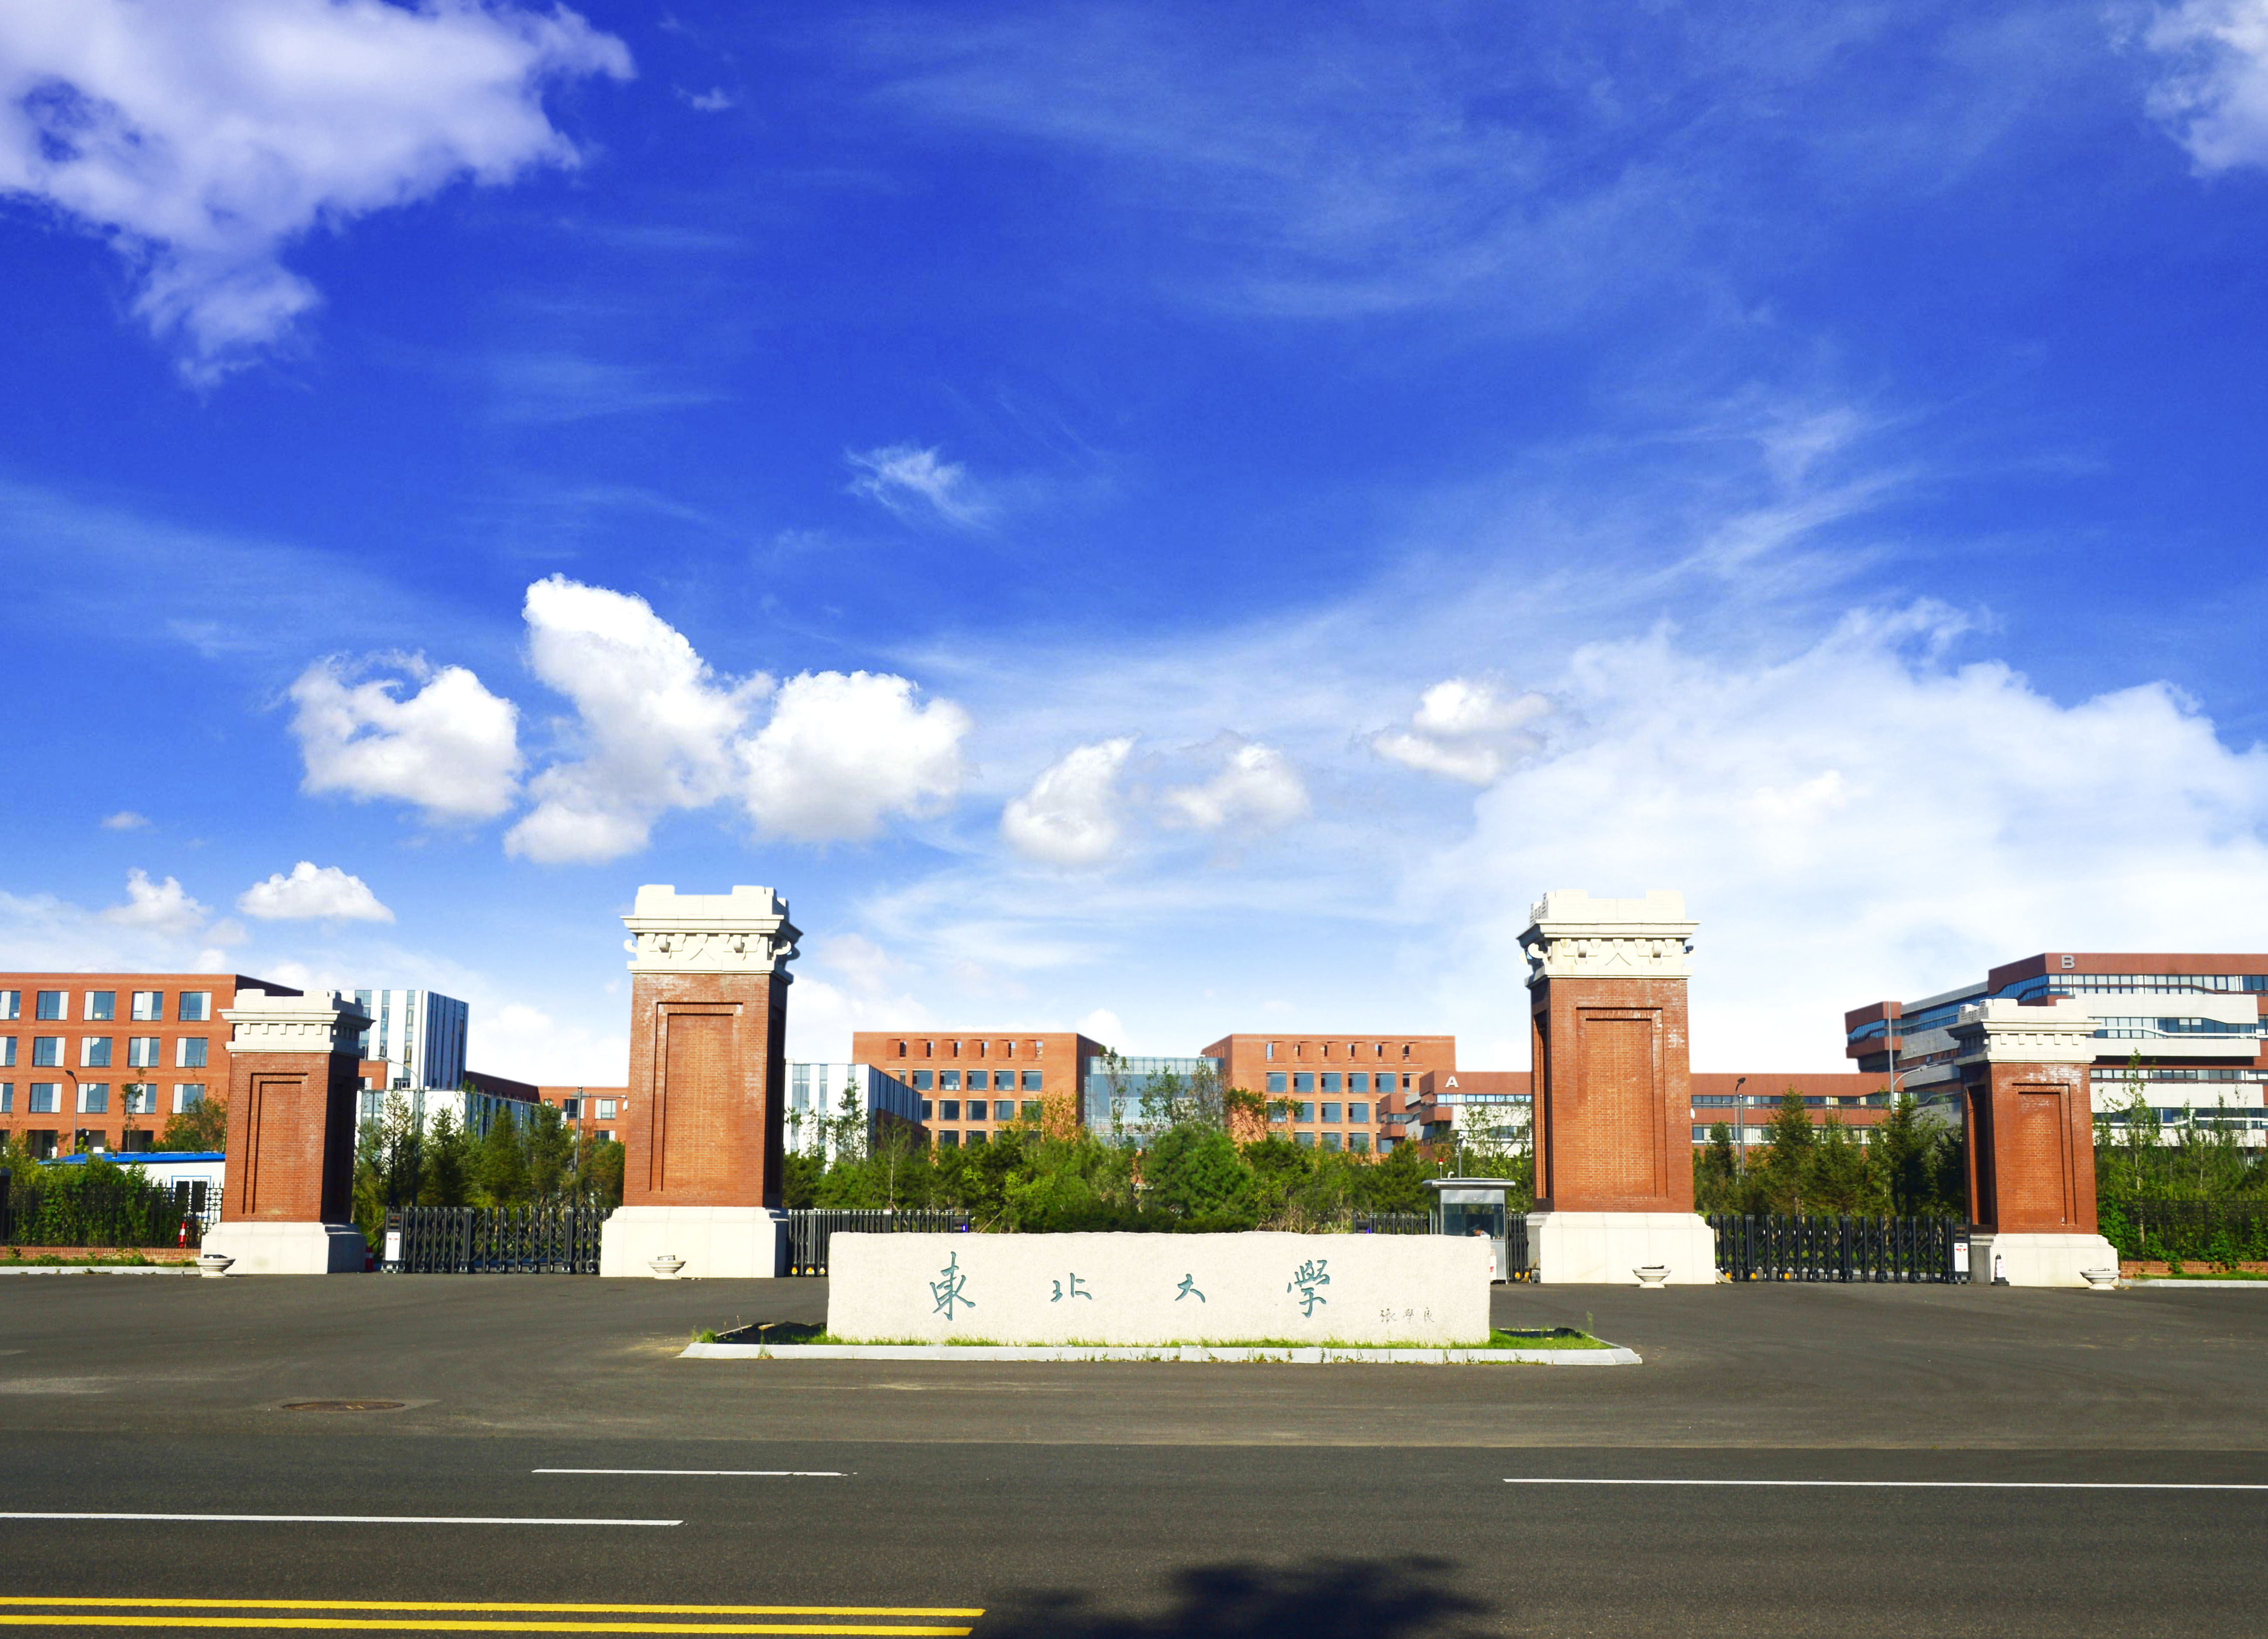
\includegraphics[width=0.8\linewidth]{img/fig1.jpg}
    \caption{一张示例图片}
    \label{fig:figure1}
\end{figure}



        \subsection{国内外研究状况}
            \subsubsection{国外研究现状}
                \xiaosi


\begin{equation}
     \sum_{i=\left\lceil\frac{m}{2}\right\rceil}^{m}\left(\begin{array}{c}
     m \\
     i
     \end{array}\right) p^{i}(1-p)^{m-i}=\sum_{i=0}^{\left\lfloor\frac{m}{2}\right\rfloor}\left(\begin{array}{c}
     m \\
     i
     \end{array}\right)(1-p)^{i} p^{m-i}
\end{equation}


\begin{equation}
    \begin{aligned}
        \operatorname{Pr}\left\{o_{k}^{*} \!\succeq \!r\! \succeq \!o_{c k}^{*} \mid x, m\right\}\!=\!1 & \!-\!\sum_{i=\left\lceil\frac{m}{2}\right\rceil}^{m}\!\left(\!\begin{array}{c}
        m \\
        i
        \end{array}\right) p^{i}(1\!-\!p)^{m\!-\!i} \\
        & \!-\!\sum_{i=\left\lceil\frac{m+1}{2}\right\rceil}^{m}\!\left(\!\begin{array}{c}
        m \\
        i
        \end{array}\right) q^{m\!-\!i}(1\!-\!q)^{i}
    \end{aligned}
\end{equation}
            \subsubsection{国内研究现状}
                \xiaosi 

\begin{enumerate}
    \item 分项1
    \item 分项2
    \item 分项3
\end{enumerate}

        \subsection{本章小结}
            \xiaosi 


\begin{figure}[H]
    \centering
    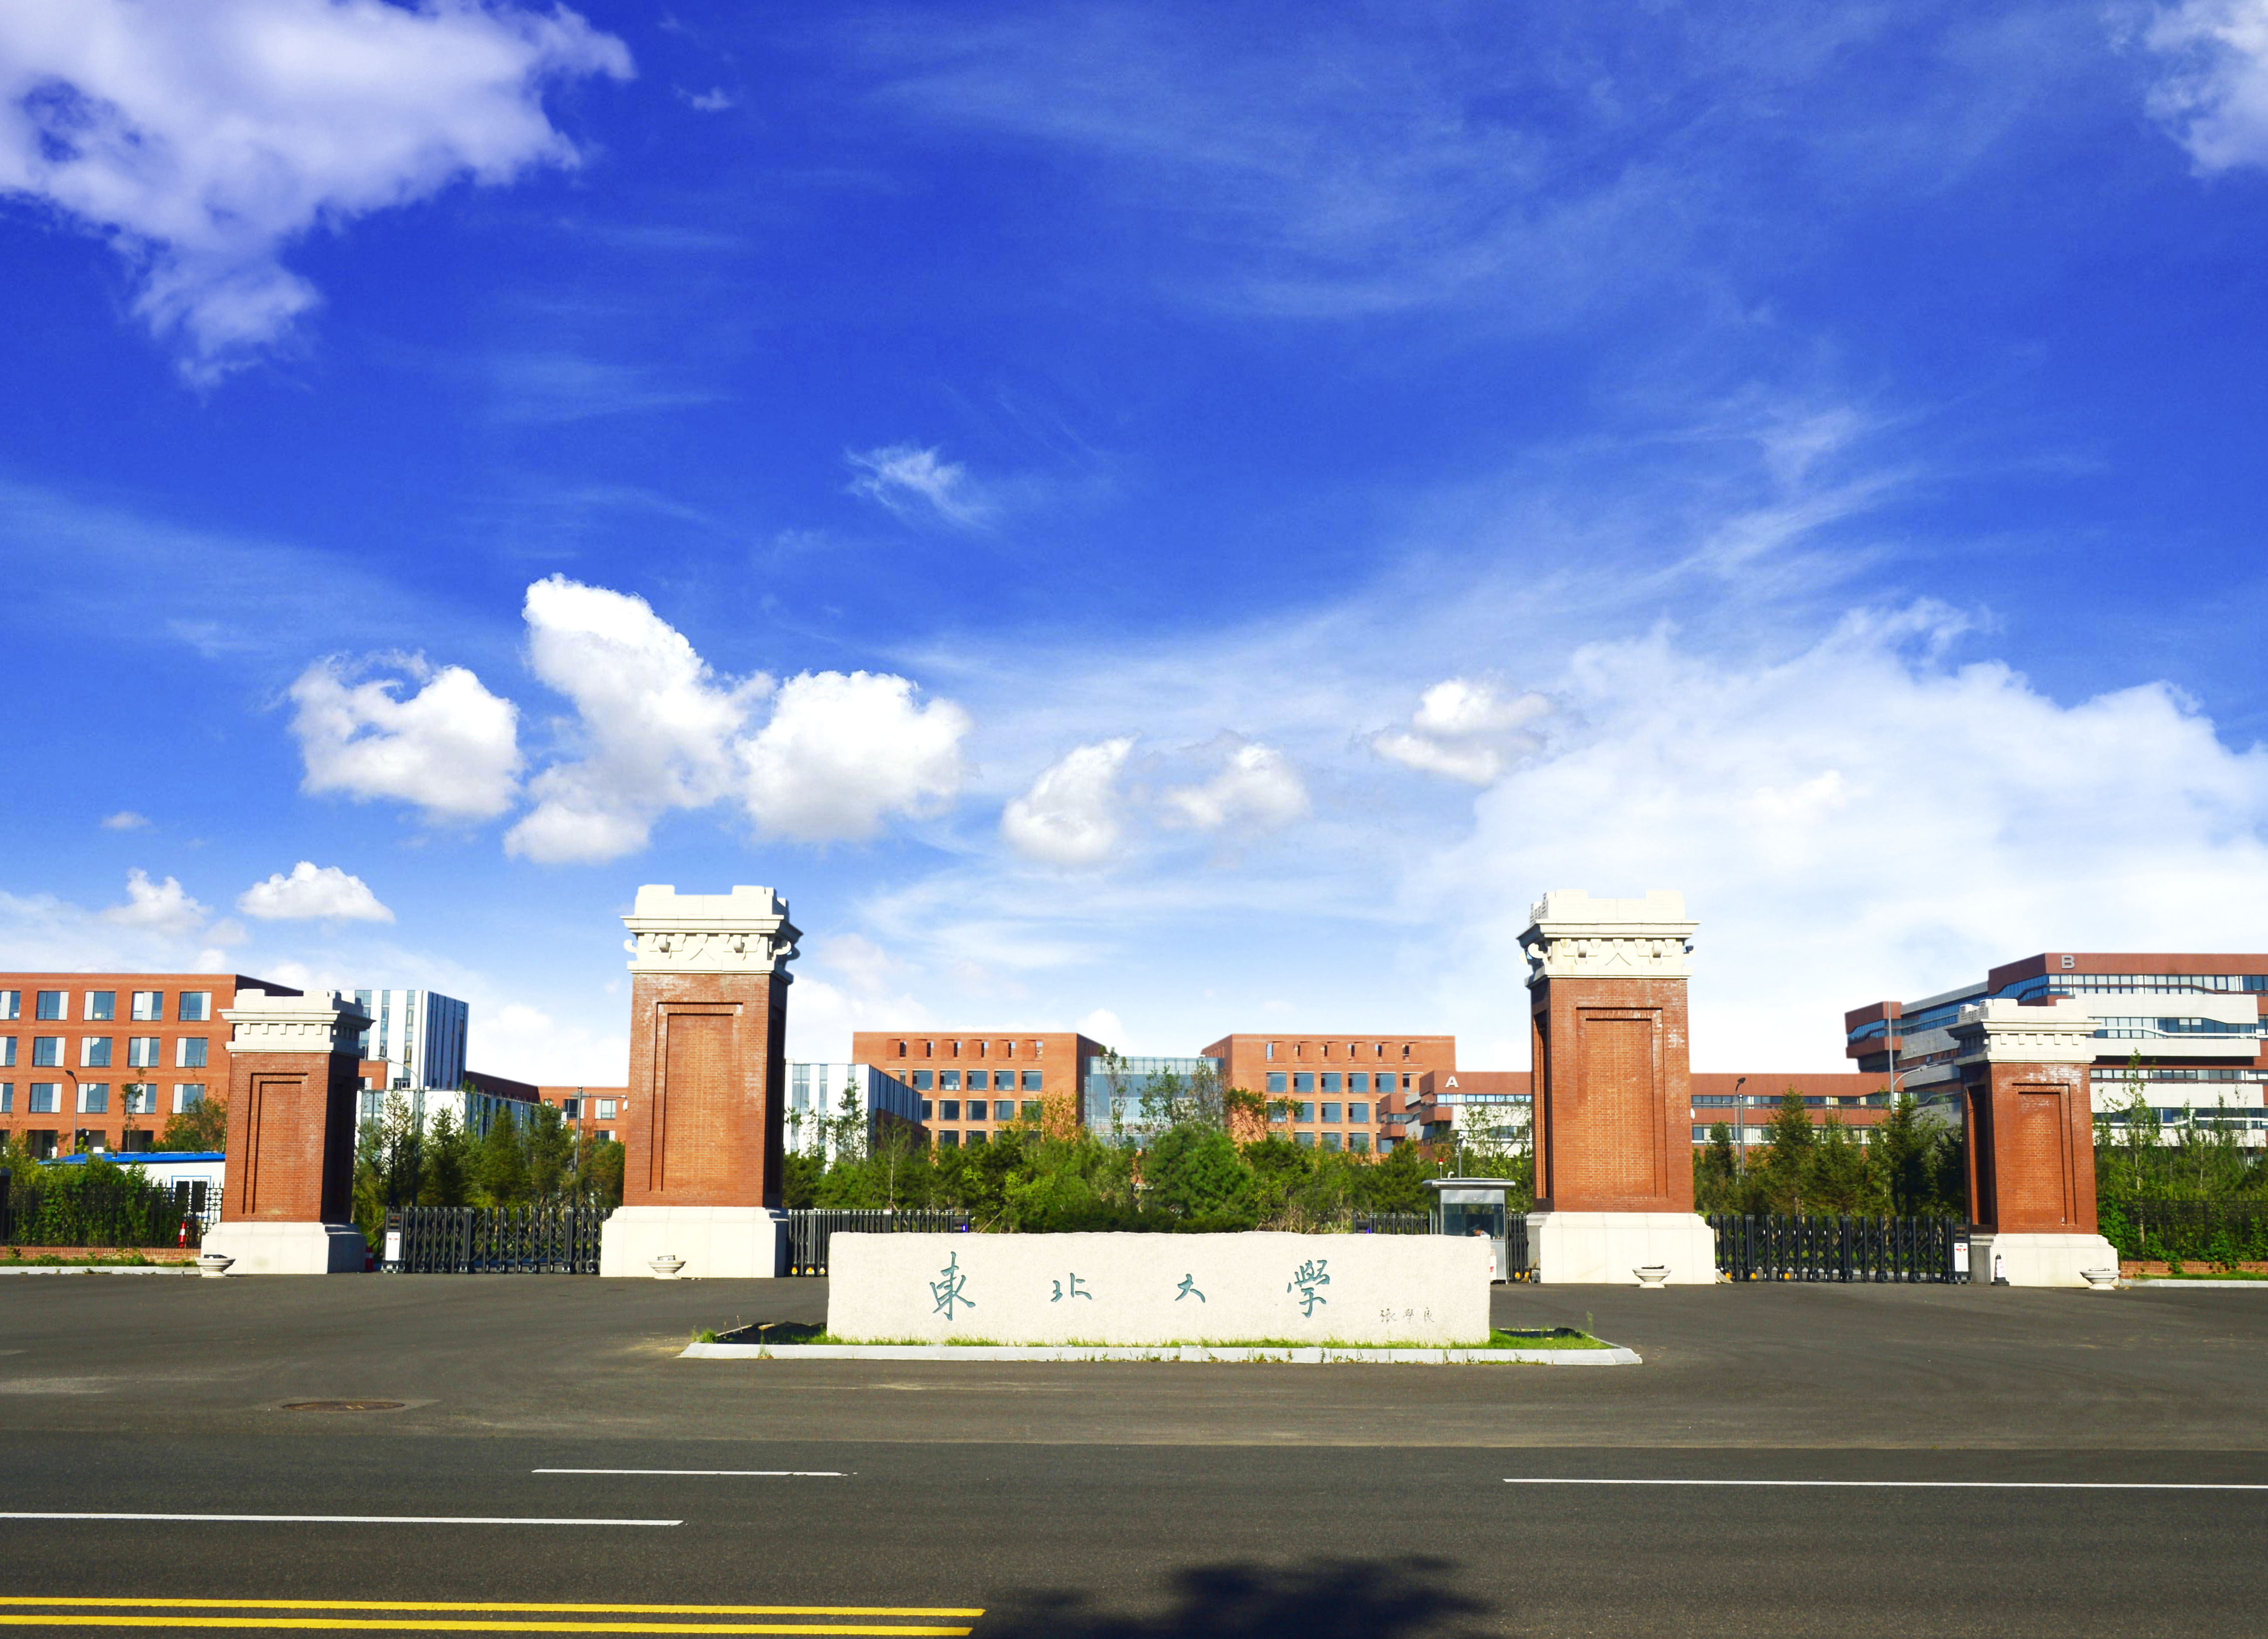
\includegraphics[width=0.8\linewidth]{img/fig1.jpg}
    \caption{注意图例图题}
    \label{fig:figure2}
\end{figure}

        \subsection{本文的研究内容和技术路线}
            \subsubsection{本文的研究内容}
                \xiaosi
本文拟通过室内实验,建立中关铁矿全尾砂胶结充填体的损伤本构方程和损伤演化方程,利用充填体与围岩的能量匹配分析得到满足中关铁矿实际开采条件的最佳强度和配比,从而降低矿山生产成本。

在室内实验研究的基础上,对中关铁矿首先开采的-230中段进行数值模拟,对其采场结构参数进行优化,得到阶段空场嗣后充填采矿法的最佳采场结构参数,为矿山的设计、生产提供依据。

本文以中关铁矿为工程背景,研究的内容主要如下:

(1)在实验室进行充填体力学实验,得到相应的物理力学参数;

(2)进行充填体的受力和损伤力学研究;

(3)充填体与采场围岩合理匹配分析;

(4)从充填体的力学特性出发,利用有限差分软件$FLAC^{3D}$,通过研究充填体的破坏指数及矿房顶底板受力、位移及塑性区等指标,优化采场结构参数。

    \clearpage
    \sanhaolineskip
    \section{相关技术介绍}
        \subsection{技术一}
            \xiaosi 

\wuhao
\begin{table}[H]
  \centering
  \caption{表格标题}
  \label{tab:my-table}
  \begin{tabular}{|c|c|c|}
    \hline
    字段名 & 字段类型 & 是否为空 \\
    \hline
    id & int & NOT NULL \\
    \hline
    name & varchar(20) & NOT NULL \\
    \hline
    age & int & NULL \\
    \hline
  \end{tabular}
\end{table}



        \subsection{技术二}
            \xiaosi


\begin{figure}[H]
    \centering
    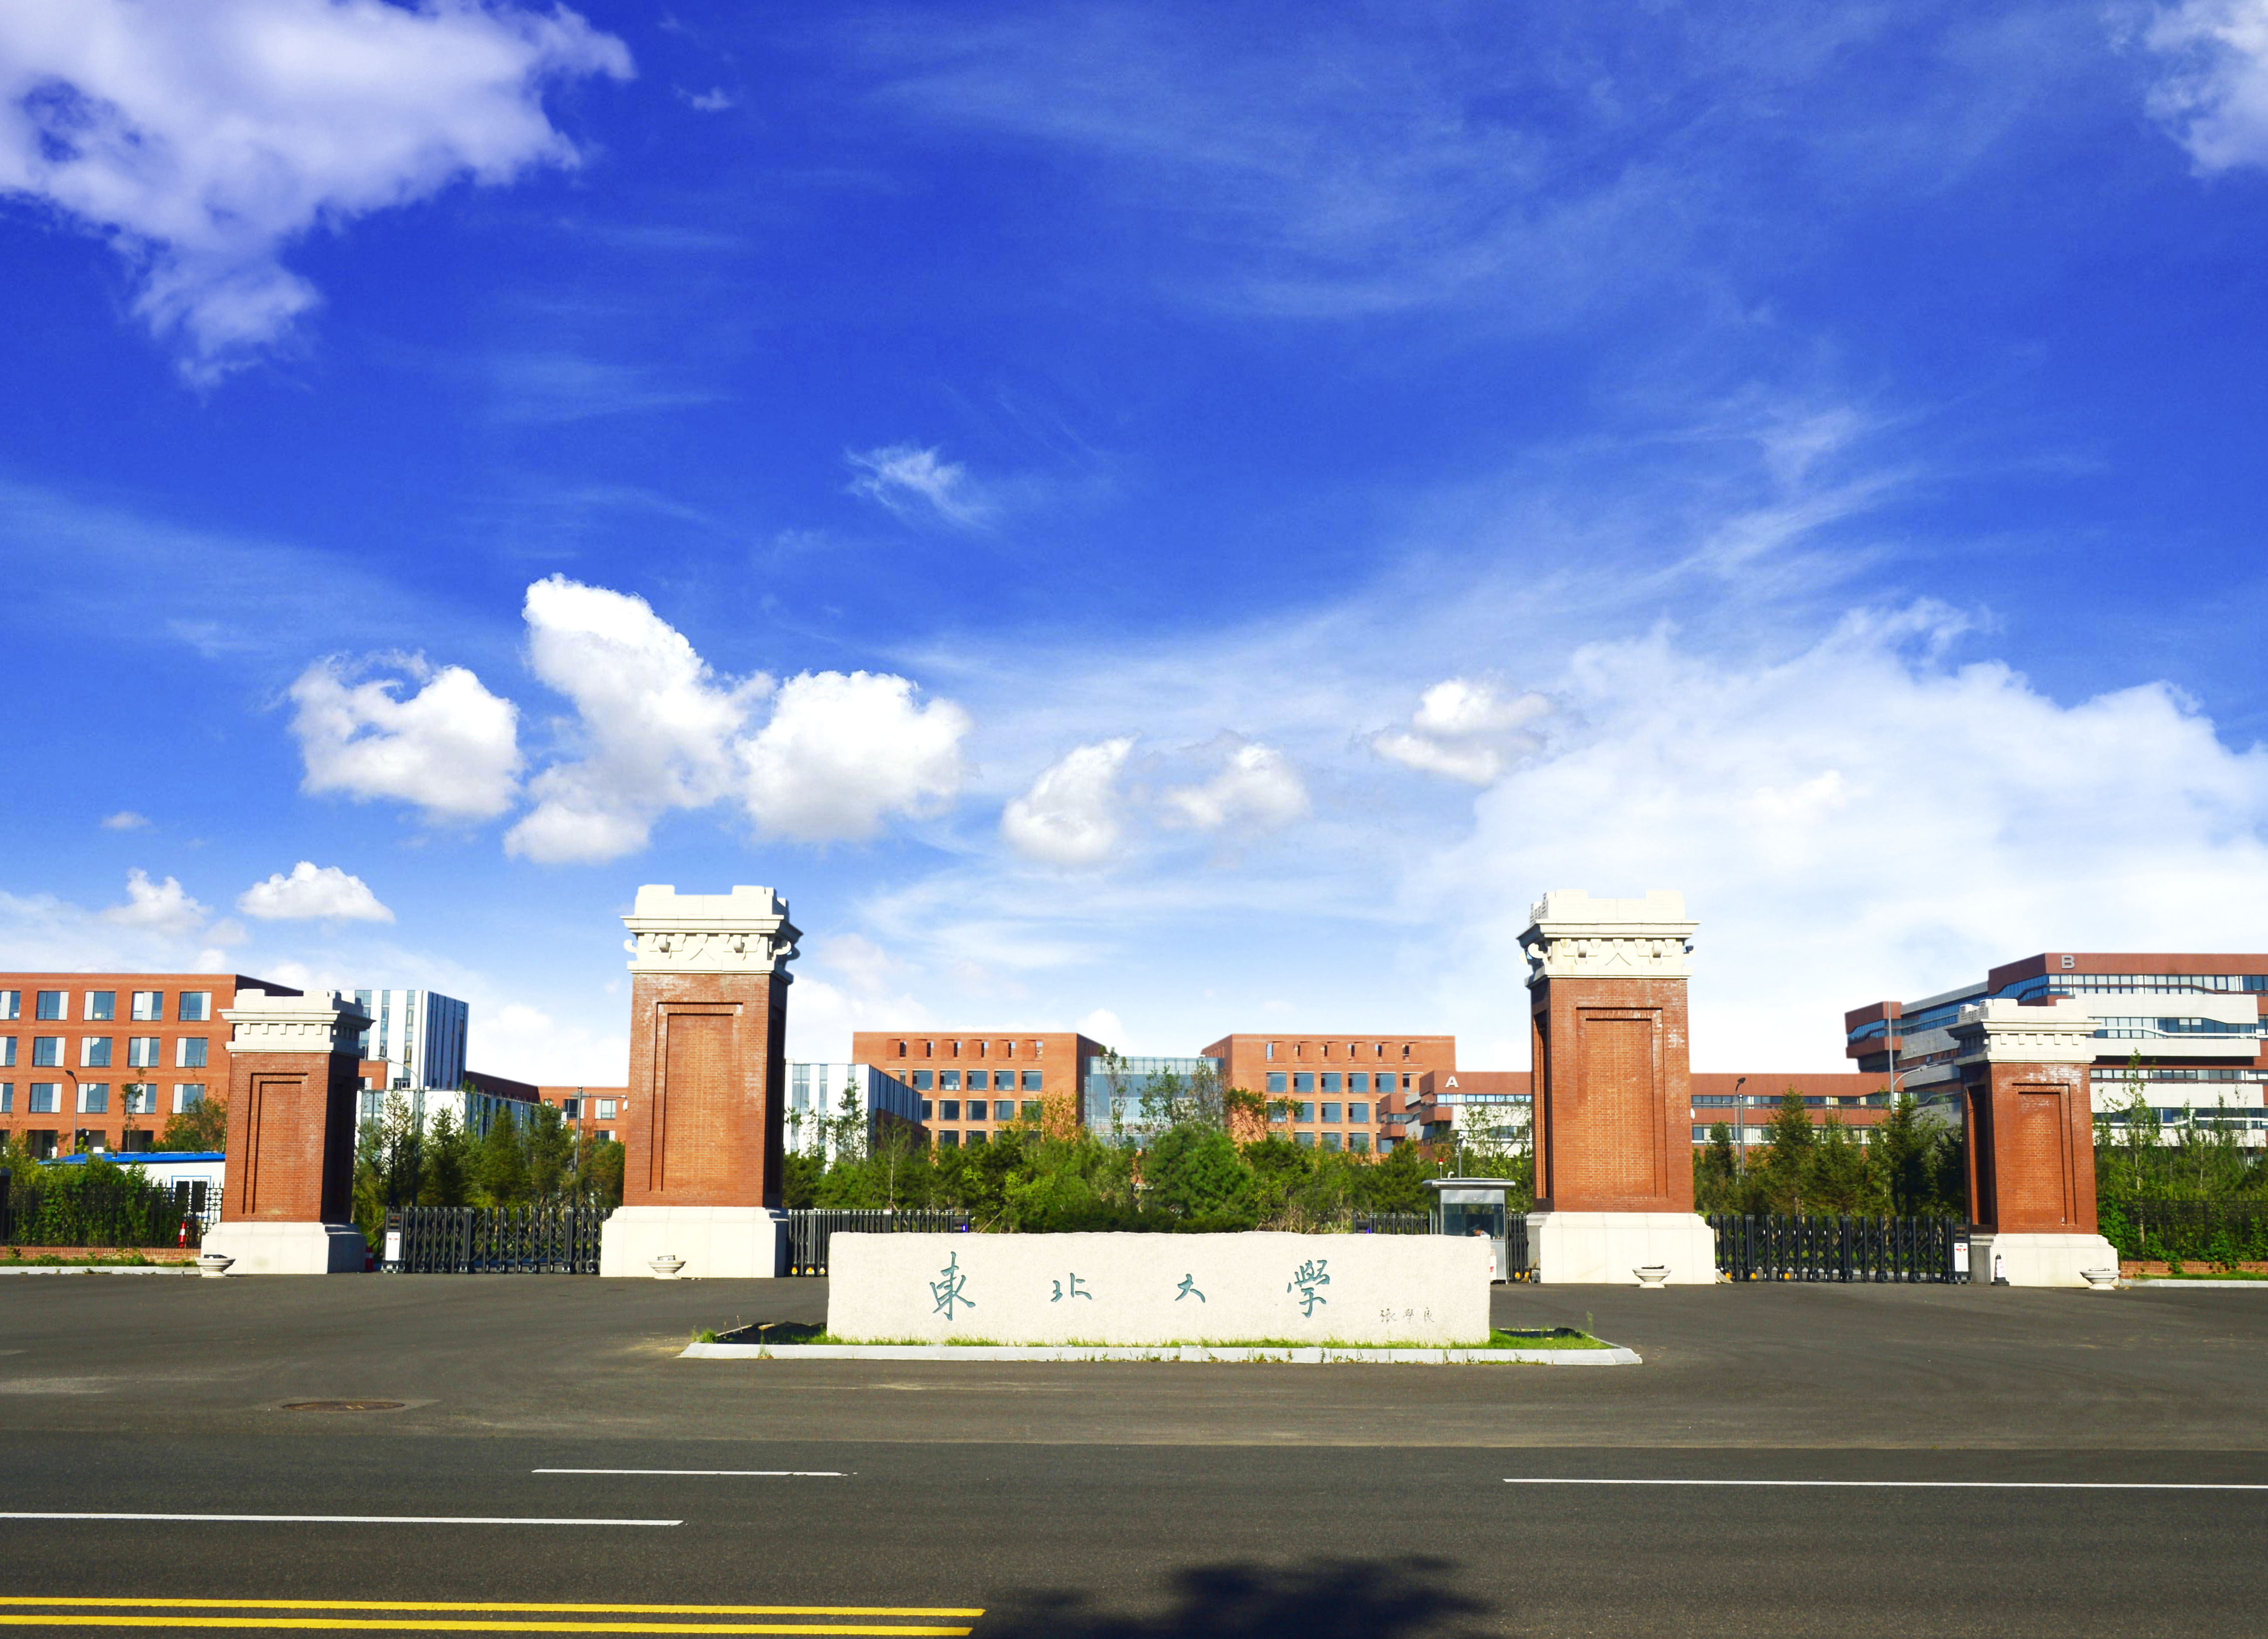
\includegraphics[width=0.8\linewidth]{img/fig1.jpg}
    \caption{一张示例图片}
    \label{fig:figure3}
\end{figure}
    % ================================================================


    % ==========================  参考文献  ==========================
    \clearpage
    \sanhaolineskip
    \bibliography{reference}
    \bibliographystyle{unsrt}
    \addcontentsline{toc}{section}{参考文献}
    % ================================================================


    % ============================ 致谢  =============================
    \clearpage
    \sanhaolineskip
    \section*{致\quad\ 谢}
        \xiaosi \song 

uu们都看到这里了,来个三连吧!
    \addcontentsline{toc}{section}{致谢}
     % ================================================================
     

    % ============================ 附录  =============================
    \clearpage
    \sanhaolineskip
    \section*{附\quad\ 录}
        
\xiaosi
这里是代码。
\lstinputlisting[
    style       =   Python,
    caption     =   {\bf example.py},
    label       =   {example.py}
]{code/example.py}
    \addcontentsline{toc}{section}{附录}
    % ================================================================

    
\end{document}
